% !TeX spellcheck = de_DE
\documentclass[fontzize=12pt,paper=a4,twoside=false]{article}
\usepackage{german}
\usepackage{graphicx}
\usepackage{fullpage}
\usepackage{hyperref}
\hypersetup{
    colorlinks=true,
    linkcolor=blue,
    filecolor=magenta,      
    urlcolor=cyan,
}
\title{Kurzwellenausbreitung}
\author{Konrad Gralher}

\begin{document}
\begin{titlepage}
    \bfseries\Huge\centering{
    Kurzwellenausbreitung\\
    Amateurfunklehgang 2021\\
    \vskip3cm
    \huge\itshape{
        Konrad Gralher\\
        }
    }    
    \begin{figure}
        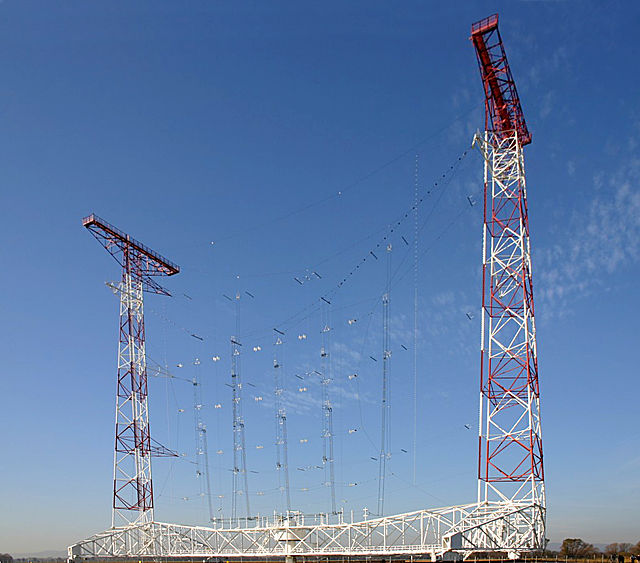
\includegraphics[]{assets/640px-Moosbrunn_SW_Antenna}
        \caption{Kurzwellenstation Moosbrunn}  
    \end{figure}        
\end{titlepage}

\part[]{Wellenausbreitung}

Die Sendungen im Kurzwellenbereich werden in der Ionosphäre reflektiert. 
Ukw besitzt diese Eigenschaften nicht, da die Wellen sich eher wie Licht ausbreiten(bedingt durch kleinere Wellenlänge). Durch Reflektionen der Kurzwelle an der Ionosphäre
sind deutlich größere Reichweiten möglich(DX Betrieb).
\vspace{0.1cm}
\subsection[]{Wellenarten}
Bei der Kurzwellenausbreitung spielen zwei Arten der Welle eine Rolle.
\begin{enumerate}
    \item Raumwelle
    \begin{itemize}
        \item bezeichnet alle sich im Raum ausbreitende Wellen(große Reichweite wenn in Skip Distanz)
        \item hat Relevanz für KW(Kurzwelle)
        \item die Ausbreitung hängt von dem Einfallswinkel der Strahlen ab 
    \end{itemize}
    \item Bodenwelle
    \begin{itemize}
        \item bezeichnet die sich am Boden mit der Erdkrümmung ausbreitende Welle (kleine Reichweite)
        \item werden mit zunehmender Frequenz gedämpft
        \item wird im Lang- und Mittelwellebereich aufgenutzt
        \item geht über den Geografischen Horizont hinaus
    \end{itemize}
\end{enumerate}
\subsection[]{Ionosphäre}
Die für die Kurzwellenausbreitung Relevanten Schichten, befinden sich etwa in 100-500km Höhe.
Dort findet eine Brechung und anschließend eine Reflektion statt.
Die Bedingungen auf den jeweiligen Bänder hängt von der Jahreszeit der Frequenz, Sonnenflecken und Tageszeit ab. 


\href{https://www.darc.de/fileadmin/filemounts/referate/ajw/Onlinelehrgang/e09/Bild9-2.gif}{Verschiedene Schichte der Ionosphäre.}
\subsection[]{Sonnenflecken}



\end{document}